 \documentclass[ %
    11pt, %
    a4paper, %
    BCOR=12mm, %
    DIV=12, %
    headsepline=true, %
    parskip=half, %
    %draft=true, %
]{article}

\usepackage[utf8]{inputenc}
\usepackage[T1]{fontenc}
\usepackage{lmodern}
%%englisches Protokoll
%\usepackage[british,UKenglish,USenglish,english,american]{babel}
% %
%%deutsches Protokoll
\usepackage[ngerman]{babel}
% %
\usepackage{amssymb,amsmath}
\usepackage{engrec}
\usepackage{enumerate}
\usepackage{empheq}
\usepackage{picins}
\usepackage{floatflt}
\usepackage{graphicx}
\usepackage{color}
\usepackage{natbib}
\usepackage{pdfpages}
\usepackage{hyperref}
\graphicspath{{Bilder/}}%% Allgemeine Bilder
\usepackage[paper=a4paper,left=25mm,right=25mm,top=25mm,bottom=25mm]{geometry}

\begin{document}


\begin{titlepage}

\begin{center}



\includegraphics[width=0.3\textwidth]{Bilder/logo}\\[1.2cm]    

\textsc{\LARGE Albert-Ludwigs-Universit\"at Freiburg}\\[1.75cm]

\textsc{\Large Physikalisches Fortgeschrittenen-Praktikum I}\\[0.75cm]



\newcommand{\HRule}{\rule{\linewidth}{0.5mm}}
\HRule \\[0.5cm]
{ \huge \bfseries Nuclear Magnetic Resonance}\\[0.5cm]

\HRule \\[1.75cm]


\begin{minipage}{0.4\textwidth}
\begin{flushleft} \large
\emph{Students:}\\
Daniel \textsc{Uhl}\\ \setlength{\parindent}{1.25cm} \& 
\setlength{\parindent}{0cm} \\ Jan P\'eter \textsc{Szabados} 
\end{flushleft}
\end{minipage}
\hfill
\begin{minipage}{0.4\textwidth}
\begin{flushright} \large
\emph{Tutor:} \\
Davide \textsc{di Stefano}\\
\end{flushright}
\end{minipage}

\vfill


{\large \today}

\end{center}

\end{titlepage}

\tableofcontents
\newpage
\section{\textsc{Aufgabenstellung}}

\pagenumbering{arabic}
\subsection*{Vermessung der Signale mit dem Oszilloskop}
Zuerst wird eines der beiden Präparate ( $^{57}Co$ oder $^{241}Am$) vermessen. Hier bei wird eine Skizze der Signale von Hand angefertigt und die Anstiegszeiten (zwischen 10 \% und 90 \% des Maximalwertes), die Abfallzeiten (90\% $\rightarrow$ 10\%) und die Signal-Amplitude vermessen.
\subsection*{Aufnehmen der Energie-Spektren}
Mit dem Multi Channel Analyser (MCA) werden nun die Energie-Spektren von $^{57}Co$ und $^{241}Am$ aufgenommen. Dabei wird das Spektrum des $^{57}Co$ mit beiden Detektoren für beide möglichen Orientierungen der Quelle gemessen. Aus dem Ergebnis dieser Messung kann nun bestimmt werden mit welchem Detektor im weiteren Versuchsverlauf für den 14,4keV-Peak oder den 122keV-Peak gemessen wird.
In der Auswertung soll eine Energie-Kalibration für den gewählten Detektor mit den charakteristischen Peaks von beiden Quellen durchgeführt werden und die Spektren der beiden Präparate anhand der Ergebnisse interpretiert werden.
\subsection*{Setzen der Energiefenster}
Die Energiefenster werden an den beiden Single Channel Analyser (SCA) jeweils für ein Signal eines 14,4keV Photons bzw. eines 122keV Photons eingestellt.
\subsection*{Messung der verzögerten Koinzidenzen}
Nun wird das Spektrum der verzögerten Koinzidenzen vermessen. Dabei gibt das 14,4keV Photon das Startsignal und das verzögerte 122keV Photon das Stoppsignal.
Ausgewertet wird einmal durch einen Fit einer Exponentialfunktion an das linear aufgetragene Spektrum und einmal durch den Fit einer linearen Funktion an das logarithmische Spektrum. Davor muss das Spektrum der zufälligen Koinzidenzen abgezogen werden, welches man durch eine Messung bestimmt bei dem das Start- und Stoppsignal vertauscht wird.
\subsection*{Zeitkalibration des TAC}
Der Time to Amplitude Converter (TAC) wird kalibriert indem man die Pulse eines Single Channel Analysers (SCA) aufteilt und eines der Signal über die Delay-Boxen verzögert. Das unverzögerte Signal wird an den Start-Eingang angeschlossen und das verzögerte an den Stopp-Eingang. Man variiert nun die Delays und nimmt zum jeweiligen Delay den jeweiligen Kanal auf welcher angesprochen wird auf.
\clearpage
\section{\textsc{Theoretische Grundlagen}}
\subsection{Radioaktive Zerfälle}
Instabile Kerne können unter Aussendung charakteristischer radioaktiver Strahlung zerfallen. Dieser Zerfall kann auf unterschiedlichen Wegen geschehen und dabei können unterschiedliche Arten von Strahlung frei gesetzt werden. Radioaktiver Zerfall ist ein statistischer Prozess, dabei ist die Änderung einer radioaktiven Probe $dN$ nach einer Zeit $t$ proportional zur gesamten Menge der Probe N:
\begin{center}
\[\frac{dN}{dt}=-\lambda N \]
\end{center}
Eine Lösung zu dieser Differentialgleichung erhält man durch separieren der Variablen und erhält durch integrieren:
\begin{center}
\[\ln N(t)-\ln N(0)= \int\limits_{N(t)}^{N(0)}\frac{dN'}{N'}=- \int\limits_{t}^{0}\lambda dt'= -\lambda t \]
\[ \Leftrightarrow \ln{\frac{N(t)}{N(0)}} = -\lambda t\]\\
\[ \Leftrightarrow N(t)= N(0) \exp(-\lambda t)\]
\end{center}
Aus dieser Formel lässt sich nun auch die Halbwertszeit $T_{\frac{1}{2}}$ berechnen:
\begin{center}
\[ \frac{1}{2}N_0 = N(T_{\frac{1}{2}}) = N_0 \exp(-\lambda T_{\frac{1}{2}})\]\\
\[ \Leftrightarrow T_{\frac{1}{2}} = \frac{\ln 2}{\lambda}\]
\end{center}
Und für die Lebensdauer gilt
\begin{center}
\[ \tau = \frac{1}{\lambda}= \frac{T_{\frac{1}{2}}}{\ln 2}~~. \]
\end{center}
\subsubsection{$\alpha$-Zerfall}
Bei schweren Kernen kann man das Phänomen des  $\alpha$-Zerfalls. Beim $\alpha$-Zerfall zerfällt der Mutterkern in den Tochterkern unter Aussendung eines Helium-4-Atomkerns:
\begin{center}
$_Z^AX \rightarrow _{Z-2}^{A-4}X+_2^4He$.
\end{center}
\subsubsection{$\beta$-Zerfall}
Es gibt drei verschiedene Arten von $\beta$-Zerfall: $\beta^+$- und $\beta^-$-Zerfall und den Elektroneneinfang (EC, Electron Capture).\\
~\\
\textbf{$\beta^+$-Zerfall:} Bei Kernen mit relativem Überschuss an Protonen kann $\beta^+$-Zerfall auftreten. Dabei wird ein Proton unter Aussendung eines Positrons und eines Neutrinos in ein Neutron umwandelt:
\begin{center}
$\mathit{_1^1p \rightarrow _0^1n + e^+ + \nu}$
\end{center}
Die Kernladung veringert sich um eins. Das Positron wird sich nach seiner Abbremsung durch Materie bald mit einem Elektron zu einem Positronium-Atom vereinigen, welches nach einer mittleren Lebensdauer von $10^{-7}$s bis $10^{-9}$s in zwei $\gamma$-Quanten zu je 511keV zerfällt.\\
~\\
\textbf{$\beta^-$-Zerfall}: Bei Kernen mit relativem Überschuss an Neutronen kann $\beta^-$-Zerfall auftreten. Hierbei wandelt sich ein Neutron in ein Proton um, unter Aussendung eines Elektrons und eines Antineutrinos, welches ein Teil der Zerfallsenergie weg trägt:
\begin{center}
$\mathit{_0^1n \rightarrow _1^1p+e^- + \overline{\nu}}$
\end{center}
Die Kernladung verringert sich um eins. Die Energie der ausgesendeten Elektronen ist kontinuierlich verteilt.\\
~\\
\textbf{Elektroneneinfang (EC, Electron Capture)}: Vor allem bei schweren Kernen mit Protonenüberschuss tritt EC auf. bei diesem Effekt wird ein Elektron aus der K-Schale vom Kern eingefangen unter Aussendung eines Neutrinos, wodurch sich die Kernladungszahl um eins verringert. Der dadurch entstandene freie Platz in der K-Schale wird durch ein Elektron aus der, meistens nächst höheren L-Schale wieder aufgefüllt. Die durch den Übergang des Elektrons in die niedrigere Schale frei werdende Energiedifferenz wird als Röntgen- oder Augerstrahlung abgestrahlt. Der freie Platz in der L-Schale wird wiederum durch ein Elektron aus einer höheren Schale besetzt. Dieser Prozess setzt sich in Richtung äußerer Schalen fort bis eine stabile Elektronenkonfiguration wieder erreicht ist. Bei diesem Vorgang wird bei jedem Elektronenübergang eine für die entsprechende Energiedifferenz charakteristische Röntgenstrahlung frei gesetzt.
\subsubsection{$\gamma$-Strahlung}
Bei der $\gamma$-Strahlung haben wir keine Veränderung bei der Nukleonenzahl oder der Kernladungszahl. Sie ist eine Begleiterscheinung der oben genannten Zerfälle. Nach einem Zerfall ist der Tochterkern meist in einem angeregten Zustand, welcher unter aussenden von $\gamma$-Quanten, mit der entsprechenden Energie, in einen tieferen Zustand zurück fällt bis er beim Grundzustand angekommen ist.
\subsubsection{Innere Konversion (IC, Internal Conversion)}
Ein zur $\gamma$-Strahlung konkurrierender Prozess ist die innere Konversion. Sie tritt vor allem bei schweren Kernen und geringer Zerfallsenergie auf. Die innere Konversion ist ein strahlungsloser Übergang eines angeregten Kernzustands in einen tieferen, hier wird die freiwerdende Energie an eines der Hüllenelektronen übertragen und dieses bei diesem Vorgang ausgesendet wird. Die Energieübertragung findet hierbei direkt statt ohne dass ein reelles $\gamma$-Quant erzeugt wird welches das Elektron später absorbiert. Diese Elektronen zeigen, im Gegensatz zum $\beta$-Zerfall, ein kontinuierliches Spektrum. Man erhält ein monoenergetisches Spektrum welches von der Schale des emittierten Elektrons abhängt. Die frei werdende Energie bei auffüllen der Lücke, durch herabfallende Elektronen in Hüllen niedrigerer Energien, wird als charakteristische Röntgenstrahlung oder durch Auger-Elektronen aufgefüllt.
\subsection{Prozesse in der Atomhülle}
Wie bereits besprochen ist die Folge eines Elektroneneinfangs oder einer inneren Konversion, ein unbesetzter Elektronen-Zustand. Dieser Zustand wird durch ein Elektron aus einer höheren Schale aufgefüllt. Durch den Übergang wird die frei werdende Energiedifferenz entweder durch Emission von charakteristischer Röntgenstrahlung oder durch ein Auger-Elektron abgeführt. Beim Effekt des Auger-Elektrons wird die Energie wie bei der inneren Konversion direkt an das Elektron einer anderen Schale übertragen, welches dann druch aus der Atomhülle geschlagen wird. Dieses Elektron nennt man Auger-Elektron. Die nun frei gewordene Lücke wird nun wieder durch ein Elektron besetzt unter Aussendung von Röntgenstrahlung oder eines Auger-Elektrons.
\subsection{Wechselwirkung von Photonen mit Materie}
Man nutzt die Wechselwirkung von $\gamma$-Quanten mit Materie um diese Nachzuweisen. $\gamma$-Strahlen befolgen bei der Absorption folgendes Exponentialgesetz:
\begin{center}
$I_d=I_0e^{\mu d}$
\end{center}
Wobei $I_0$ der Intensität vor dem absorbierenden Material entspricht, $I_d$ der Intensität bei einer Eindringtiefe $d$ und $\mu$ ist der Absorptionskoeffizient der absorbierenden Materie. Dieser Koeffizient hängt sowohl von $E_{\mu}$ als auch vom Absorber-Material ab.
Es gibt im Wesentlichen drei Wechselwirkungs-Mechanismen von $\gamma$-Quanten mit Materie deren Wirkungsquerschnitt mit der $\gamma$-Energie $E_{\gamma}$ und der Kernladungszahl $Z$ des Materials abhängt:
\subsubsection{Photoeffekt}
Der Photoeffekt tritt vor allem bei einer Energie $E_{\mu}$ < 200 keV (bei $Z \approx 50$) auf. Beim Photoeffekt überträgt ein $\gamma$-Quant seine Energie vollständig an ein Elektron, worauf dieses aus der Atomhülle geschlagen wird und erhält kinetische Energie. Die frei Stelle in der Atomhülle wird durch ein Elektron aus einer höheren Schale besetzt was zu den oben genannten Effekten führt.
\subsubsection{Comptoneffekt}
Der Comptoneffekt tritt überwiegend bei einer Energie von 200 keV < $E_{\gamma}$ < 5 MeV auf. Beim Comptoneffekt gibt ein $\gamma$-Quant beim Zusammenstoß mit einem Elektron nur ein Teil seiner Energie an das Elektron ab. Es wird an dem Elektron gestreut.

\begin{figure}[h]
\begin{center}
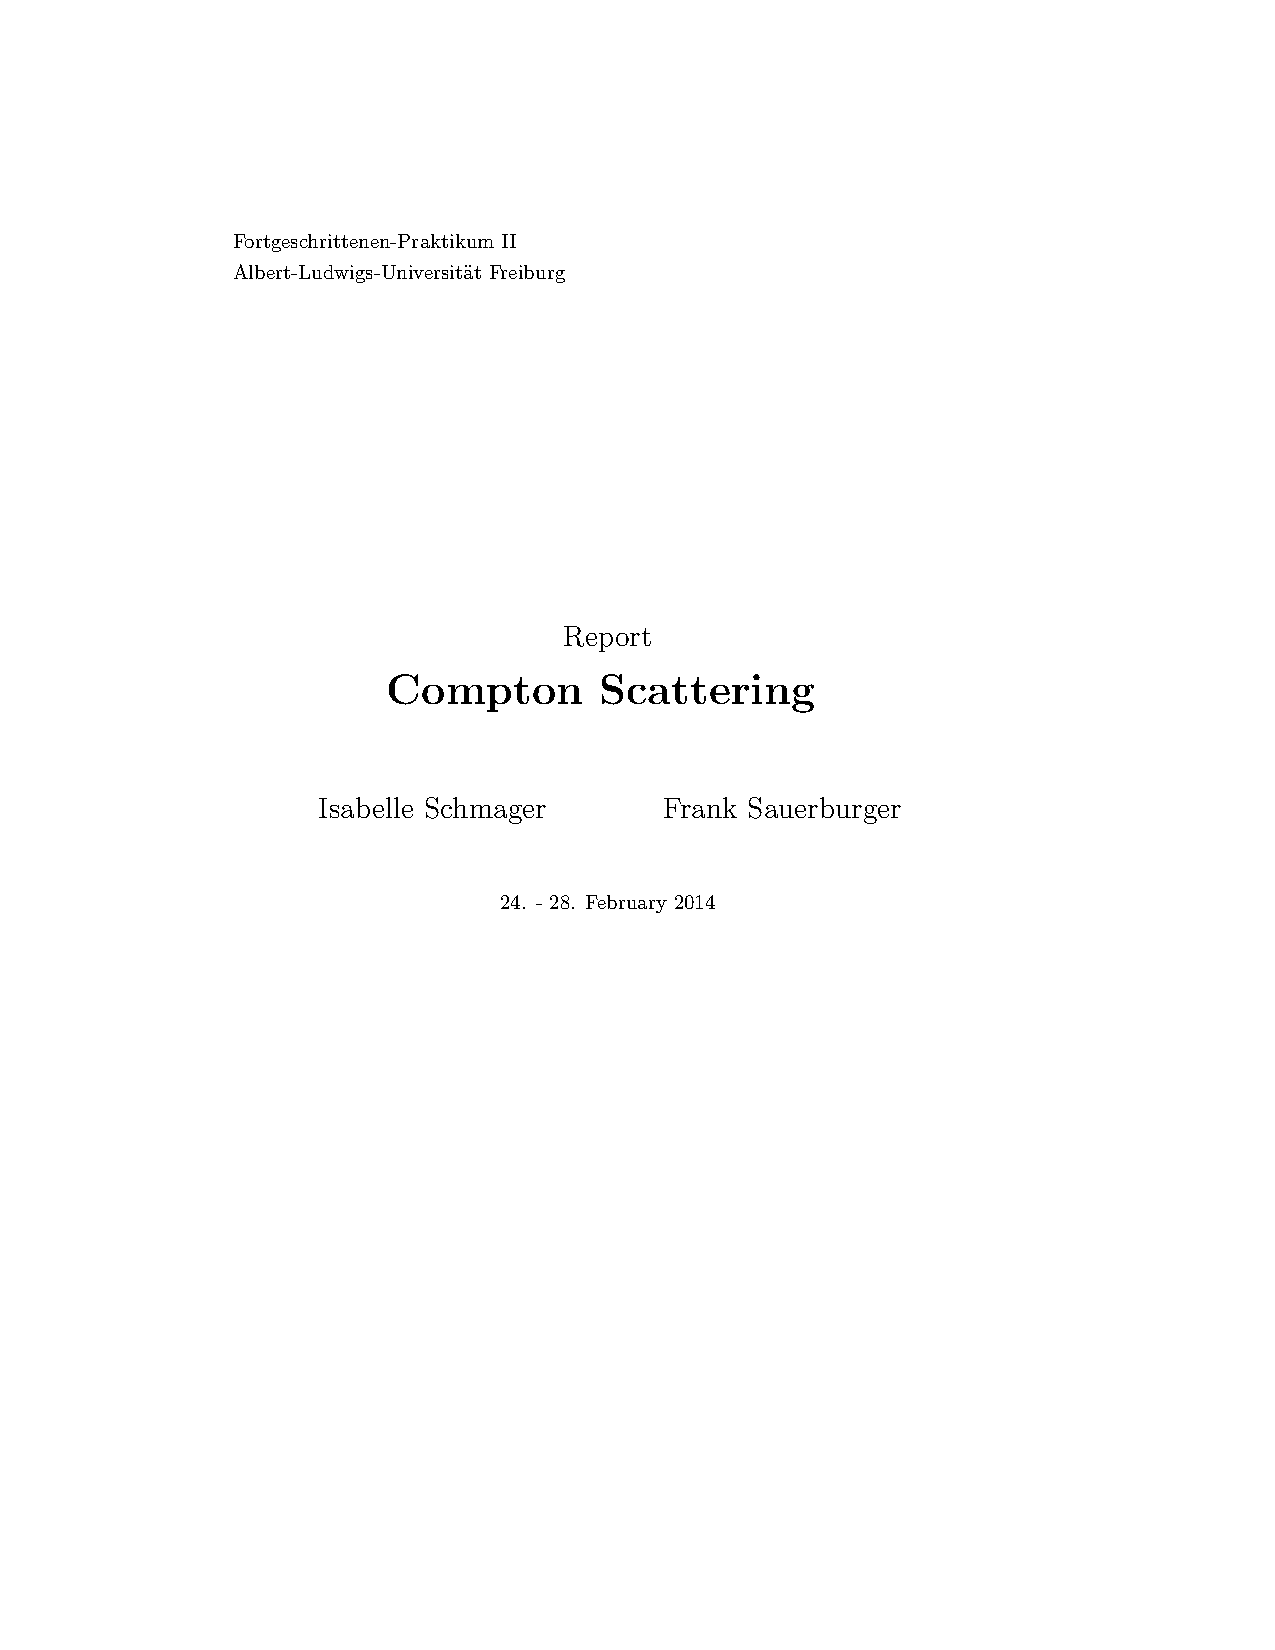
\includegraphics[scale=0.25]{compton}
\caption{Schema zum Comptoneffekt. Quelle: [ung]}
\label{fig:graph1}
\end{center}
\end{figure}

\subsubsection{Paarbildung}
Paarbildung beobachtet man ab einer Energie $E_{\gamma} \ge$ 1,022 MeV. Paarbildung erhält man, wenn ein $\gamma$-Quant mit einem elektromagnetischen Feld eines Atomkerns oder eines Elektrons in Wechselwirkung tritt. Dabei wird das $\gamma$-Quant vollständig absorbiert und ein Positron-Elektron-Paar entsteht. Die Energie des $\gamma$-Quants wird auf die beiden Teilchen verteilt und der überschüssige Impuls wird vom Kern aufgenommen. Das Positron zerfällt zu zwei $\gamma$-Quanten mit je 0,511 MeV, da es nicht lange existieren kann und sich mit einem Elektron vereint.
\subsection{Elektronik zum Nachweis vom $\gamma$-Quanten}
\subsubsection{Szintillator}
Um $\gamma$-Quanten zu detektieren benutzen wir einen Szintillator. Generell unterscheidet man hier zwischen zwei Arten von Szintillatoren, den anorganischen und den organischen. In unserem Aufbau wird ein anorganischer Szintillator benutzt.\\
Im Gegensatz zu den organischen, bei denen die einzelnen Moleküle eine Rolle spielen, spielt bei den anorganischen das Gitter des Ionenkristalls eine Rolle. Bei beiden Arten erhält man jedoch durch die Interaktion von einem $\gamma$-Quant mit dem Detektormaterial eine Lichtemission. Dabei wird ein $\gamma$-Quant mit hoher Energie umgewandelt zu einem oder mehreren mit geringerer Energie, durch den Photo- oder Comptoneffekt. Unsere Szintillator enthält einen NaI(Ti)-Kristall, die Dotierung mit Titan sorgt für weitere Energieniveaus in der Bandlücke des reinen NaI-Kristalls und somit, dass die Quanten mit bereits kleinerer Energie nicht wiederholt vom Kristall absorbiert werden.
\subsubsection{Photomultiplier}
Der Photomultiplier wandelt Lichtimpulse, in unserem Fall die vom Szintillator zugeleiteten, umzuwandeln in zur Lichtintensität proportionale elektrische Impulse umzuwandeln und diese durch Elektronenvervielfachung zu verstärken. Zum Umwandeln des der Lichtimpulse wird eine Photokathode benutzt. An ihr schlagen die ankommenden $\gamma$-Quanten, durch den Photoeffekt, Elektronen heraus. Ein $\gamma$-Quant kann mehrere Elektronen aus der Photokathode heraus schlagen welche durch eine anliegende Spannung zu ersten Dynode beschleunigt und befreien dort beim aufschlagen mehrere Sekundärelektronen, welche zur zweiten Dynode beschleunigt werden. Dies wiederholt sich bei allen weiteren Dynoden, da bei diesen sich jeweils die Spannung erhöht.

\begin{figure}[h]
\begin{center}
\includegraphics[scale=1.0]{PM}
\caption{Prinzipielle Funktionsweise eines Photomultipliers. Quelle: [hep].}
\label{fig:PM}
\end{center}
\end{figure}



\clearpage
\section{\textsc{Versuchsaufbau und Durchführung}}
\subsection{Vermessung der Signale am Oszilloskop}
Um die Signale mit dem Oszilloskop vermessen zu können, wurde es einmal direkt an den Photomultiplier (an den Preamplifier) angeschlossen und am Mainamplifier jeweils einmal am bipolaren und am unipolaren Ausgang.
\subsection{Aufnehmen der Energie-Spektren}
Hierzu wurde der unipolare Ausgang des MP mit dem Vielkanalanalysator (Multi Channel Analyser, MCA) verbunden, siehe Abbildung \ref{fig:spek_auf}. Die Spektren werden als Histogramm auf dem Computer aufgenommen, der MCA ordnet jedem Eingangsimpuls abhängig von dessen Pulshöhe einen Kanal zu. Um die Spektren interpretieren zu können werden die wird eine Energie-Eichung des MCAs durchgeführt, indem man Gauß-Kurven an die charakteristischen Peaks fittet und ermittelten Kanalnummern der Peaks gegen die Energie der Peaks aufträgt. Dieser Zusammenhang sollte linear sein.

\begin{figure}[h]
\begin{center}
\includegraphics[scale=0.25]{energiespektren}
\caption{Schaltschema zum Aufnehmen der Energiespektren. Quelle: [ver]}
\label{fig:spek_auf}
\end{center}
\end{figure}
\subsection{Setzten der Energiefenster}
An einem Singel Channel Analyser (SCA) kann man ein Energiefenster angeben, dieser gibt dann nur Signale aus wenn ein Signal welches in diesem entsprechenden Energiefenster liegt bei ihm ankommt. Diese ist unabhängig von der Signalhöhe, man erhält somit nur die Information, dass ein Signal in diesem Fenster detektiert wurde. Nun wird das Energiefenster des einen SCA auf den Peak bei 14,4 keV (späteres Start-Signal) und das andere auf 122 keV (späteres Stopp-Signal) eingestellt werden für die Messung der verzögerten Koinzidenzen. Hier sollte beachtet werden, dass die Fenster nicht zu groß und nicht zu klein gewählt werden da sonst ungewollte Nebeneffekte dominierend auftreten. Der Aufbau wird wie in Abbildung \ref{fig:energiefenster} gesteckt.
\begin{figure}[h]
\begin{center}
\includegraphics[scale=0.2]{energiefenster}
\caption{Schaltschema zum Einstellen der Energiefenster. Quelle: [ver]}
\label{fig:energiefenster}
\end{center}
\end{figure}
Bei diesem Aufbau leitet das Linear Gate die unipolaren Signal des MA nur an das MCA weiter, wenn ein Signal aus dem am SCA gewählten Energiefenster am SCA ankommt. Es muss darauf geachtet werden, dass das Delay am SCA auf den kleinsten Wert eingestellt wird damit die Signale von MA und SCA gleichzeitig beim Linear Gate ankommt und das MA Signal transmittiert wird.
\subsection{Messung der verzögerten Koinzidenzen}
Der Aufbau wird wie in Abbildung \ref*{fig:verzoegertauf} geschallten. Am TAC werden 5 $\mu s$ Eingestellt. Das 122keV-Signal soll durch die drei Delayboxen und die Verbindungskabel so verzögert werden, dass der Peak des Zeitspektrums etwa bei 4/5 des MCA-Kanalbereichs liegt. Falls nach mehreren Minuten noch keine Anzeichen von einem Peak zu erkennen so müssen die Einstellungen noch einmal geprüft werden. Ist jedoch ein Peak zu erkennen so soll die Messung mindestens 12 Stunden laufen. 
Aus dem Spektrum soll die Lebensdauer bzw. die Halbwertszeit des 14,4keV-Zustandes ermittelt werden. Beim linear aufgetragen Spektrum wird dies durch einen exponentiellen Fit und beim logarithmisch aufgetragen Spektrum durch einen Linearen Fit bestimmt. Jedoch soll vor dem Fitten der im nächsten Schritt gemessene Untergrund von den Messwerten abgezogen werden. 

\begin{figure}[h]
\begin{center}
\includegraphics[scale=0.2]{verzoegertauf}
\caption{Schaltschema zum Messung der verzögerten Koinzidenzen. Quelle: [ver]}
\label{fig:verzoegertauf}
\end{center}
\end{figure}

\subsection{Messung der zufälligen Koinzidenzen}
Bei der Messung der zufälligen Koinzidenzen wird der selbe Aufbau wie bei den verzögerten Koinzidenzen benutzt, jedoch wird das Delay auf das 122keV Signal auf Null gesetzt und das vom 14,4keV auf einige hundert ns. Die Messung sollte einige Stunden dauern.
\subsection{Zeitkalibration des TAC}
Durch den Zeit-Impulshöhen-Konverter (Time to Amplitude Converter, TAC) erhält man durch ein Rechtecksignal die Zeitdifferenz zwischen Start- und Stoppsignal, welche durch die Höhe des Pulses ausgedrückt wird. Durch das erste Signal wird die Uhr gestartet, durch das Zweite wird die Uhr gestoppt. Da das MCA nur verschieden Energieniveaus erhält wird eine Zeitkalibration des TAC benötigt, damit den Kanälen die Zeitdifferenzen zugeordnet werden können.\\

Der Aufbau zur Zeitkalibration soll wie in Abbildung \ref{fig:aufbau_kal} erfolgen. Wie in der Skizze gezeigt wird das Ausgangssignal am SCA mit einem T-Stecker aufgeteilt. Dabei wir eines direkt an das Start-Eingang des TAC gelegt das andere wird über die Delayboxen an den Stopp-Eingang gelegt. Nun wird eine Messung zu verschiedenen Delayzeiten durchgeführt, wobei der Delay und die jeweils zum Delay ansprechenden Kanäle notiert werden (dies sind meistens nur ein oder zwei Kanäle), siehe Anhang, Abbildung \ref{fig:mess_kal}. Bei der Gegenüberstellung von Kanal zur entsprechenden Verzögerung sollte ein lineare Zusammenhang deutlich zu sehen sein. Dieser wird grafisch dargestellt.\\
\begin{figure}[h]
\begin{center}
\includegraphics[scale=0.2]{aufbau_kal}
\caption{Funktionsweise des TAC. Quelle: [ver]}
\label{fig:aufbau_kal}
\end{center}
\end{figure}\\
\clearpage
\section{\textsc{Auswertung}}
\subsection{Vermessung der Signale am Oszilloskop}
Die erste Aufgabe war, die Signale des Verstärkers und des Szintillators mit dem Oszilloskop aufzunehmen. Die Zeichnungen, welche wir zu den Signalen anfertigten, finden sich im Anhang. Für das Signal des Vorverstärkers erhielten wir wie erwartet einen sehr steilen, fast senkrechten Anstieg, gefolgt von einer langen Abfalldauer. Für den unipolaren Ausgang des Hauptverstärkers erhielten wir einen positiven Peak. Als Anstiegszeit konnten wir $0,8 \mu s$, als Abfallzeit $1,5 \mu s$ bestimmen. Das Signal hatte eine Amplitude von etwa $7,8 V$. \\
Für den bipolaren Ausgang des Hauptverstärkers konnte - wie es auch der Fall sein sollte - ein positiver Peak, gefolgt von einem negativen Peak beobachtet werden. Wir vermaßen dabei die Anstiegs- und die Abfallzeit nicht, da nur der Nulldurchgang des Signals von Bedeutung ist.\\
\subsection{Spektren von $^{57}Co$ und $^{241}Am$}
Um eine Energiekalibrierung für den Multi Channel Analyzer (MCA) durchführen zu können, nahmen wir für die oben genannten Stoffe ein Energiespektrum auf, um dann die bekannten Energien der Peaks bestimmten Kanälen zuordnen zu können. Da  wir zwei Szintillatoren zur Verfügung stehen hatten, sowie zwei Ausrichtungen der Probe möglich waren, nahmen wir für $^{57}Co$ zunächst für jede Kombination von Ausrichtung und Szintillator ein Energiespektrum auf:\\
\begin{figure}[h] 
\includegraphics[scale=0.5]{coliszli}
\caption{Szintillator links, Öffnung $^{57}Co$ links}
\end{figure} \\
\begin{figure}[h]
\includegraphics[scale=0.5]{coliszre}
\caption{Szintillator rechts, Öffnung $^{57}Co$ links}
\end{figure}
\begin{figure}[h]
\includegraphics[scale=0.5]{coreszli}
\caption{Szintillator links, Öffnung $^{57}Co$ rechts}
\end{figure}
~\clearpage
\begin{figure}[h] 
\includegraphics[scale=0.4]{coreszre}
\caption{Szintillator rechts, Öffnung $^{57}Co$ rechts}
\end{figure} 
Wir befanden die Ausrichtung \glqq Szintillator rechts, Öffnung rechts\grqq für die beste, da hier auch die Nebenpeaks gut ausgeprägt sichtbar waren. Aus diesem Grund führten wir für diese Messreihe eine Anpassung an dem bekannten 122,1 keV-Peak durch: Wir benutzten dabei einen Gauss-Fit. Das Ergebnis ist, wie am $\chi^2/dof$-Wert (dof steht für \glqq degrees of freedom\grqq, also Freiheitsgrade) ablesbar, sehr gut (der Wert ist sehr nah an 1). \\
Für $^{241}Am$ führten wir nur noch eine Messung mit der oben genannten Ausrichtung durch. Dabei erhielten wir folgendes Spektrum:
\begin{figure}[h] 
\includegraphics[scale=0.4]{amreszre}
\caption{Energiespektrum $^{241}Am$}
\end{figure}
\clearpage
Der 59,5 keV-Peak ist sehr klar auszumachen (roter Gauss-Fit). Bei niedrigeren Kanal-Zahlen lässt sich außerdem etwas wie ein doppelter Peak erahnen: Hierbei überschneiden sich die Signale des 26,3- und des 33,2 keV-Peaks. Aus diesem Grund wählten wir als Fitfunktion in diesem Bereich einen sogenannten \glqq Bigaussian\grqq, also eine doppelte Gauss-Funktion. Wie man an dem $\chi^2/dof$-Wert, welcher sehr nahe an 1 liegt, sieht, handelt es sich hierbei um eine gute Fitmethode. Selbiges gilt für den 59,5 keV-Peak.\\
Für die Zuordnung der Kanäle zu den bekannten Energien erhielten wir somit: \\
\begin{table}[htbp]
\caption{}
\begin{tabular}{rrr}

\multicolumn{1}{l}{Energie in keV} & \multicolumn{1}{l}{Kanal} & \multicolumn{1}{l}{Fehler Kanal} \\ 
26,3 & 92,0 & 0,2 \\ 
33,2 & 212,9 & 0,6 \\ 
59,5 & 408,46 & 0,02 \\ 
122,1 & 833,97 & 0,18 \\ 
\end{tabular}
\end{table} \\
Obwohl Kanäle diskret und äquidistant verteilt sind und ihnen natürliche Zahlen zugeordnet sind, haben wir uns entschlossen, hier den genauen Erwartungswert der Gauss-Fits mitsamt Fehler zu verwenden, um die Genauigkeit der Kalibrierung so groß wie möglich zu halten. Es ist anzumerken, dass aufgrund der Tatsache, dass hier eventuelle Fehler der involvierten Teile des Aufbaus vernachlässigt wurden, der Fehler größer sein dürfte als aus dem Fit berechnet. \\
Die Zuordnung Kanal - Energie erfolgt im MCA linear. Aus diesem Grund benutzten wir einen linearen Fit, welcher folgendermaßen aussieht: \\
\begin{figure}[h]
\includegraphics[scale=0.5]{energiefit}
\caption{Energiekalibrierung}
\end{figure}\\
Die Werte liegen nicht genau auf einer Geraden, was angesichts der Tatsache, dass die Fehler vernachlässigt wurden und jedes Spektrum nur einmal vermessen wurde, nicht überraschend ist. 
\subsection{Verzögerte Koinzidenzen}
\subsubsection{Zeitkalibrierung des TAC}
Für die Messung der verzögerten Koinzidenzen haben wir wie auch für die nachfolgende Messung der zufälligen Koinzidenzen einen \glqq Time-to-Amplitude Converter\grqq (TAC) verwendet. Dieser transformiert eine Zeitverzögerung in eine Spannung, welche vom MCA gemessen und einem Kanal zugeordnet werden kann. Um einen Zusammenhang zwischen der Zeitverzögerung und dem der Spannung zugeordneten Kanal bestimmen zu können, stellten wir unterschiedliche Verzögerungen ein und schrieben uns den zugeordneten Kanal auf (für die Messwerte s. Anhang). Dabei entschieden wir uns, obwohl für manche Verzögerungen nicht nur bei einem Kanal ein Signal registriert wurde, sondern bei zweien, jeweils das Signal mit der größeren Anzahl an Counts zu verwenden (unterstrichene Werte im Anhang). Schließlich trugen wir die Verzögerungen über die Kanäle auf und verwendeten, um eine Kalibrierung zu bekommen, einen linearen Fit:\\
\begin{figure}[h]
\includegraphics[scale=0.5]{delayfit}
\caption{Kalibrierung der Verzögerung}
\end{figure}\\
Dabei erhielten wir für die Steigung:\\
$b=(0,2686\pm0,0009)\frac{ns}{Kanal}$\\
Wie der negative Offset vermuten lässt, ist allerdings die tatsächliche Verzögerung größer als die durch das Gerät und die verwendeten Kabel verwendete. Dies ist für unsere Auswertung aber nicht von Bedeutung, da nur die Steigung eine Rolle spielt. Für diese ist der Fehler wohl zu klein berechnet, da für die eingestellten Verzögerungen keine Fehler angenommen wurden. Der Fit selbst ist mit einem $\chi^{2}/dof$ von nahezu 1 sehr gut. \\
\subsubsection{Halbwertszeitbestimmung - Exponentielle Methode}
Aufgrund möglicher zufälliger Koinzidenzen, welche in diesem Versuch den Untergrund ausmachen, musste unsere Messung der verzögerten Koinzidenzen von diesen bereinigt werden. Um das tun zu können, haben wir aufgrund der unterschiedlichen Messdauer die Counts der Messung der zufälligen Koinzidenzen jeweils mit einem Vorfaktor $\frac{t_{v}}{t_{z}}$ multipliziert (dabei ist die Messdauer der zufällgen Koinzidenzen $t_{z}=6333 s$ und die der verzögerten Koinzidenzen $t_{v}=58886 s$).\\
$\Rightarrow N=N_{v}-\frac{t_{v}}{t_{z}}*N_{z}$\\
Der so erstellte Graph sollte für den ansteigenden Teil mit einer Exponentialfunktion der Form $N=y_{0}+A*e^{R_{0}*Kanal}$ modelliert werden. \\
\begin{figure}[h]
\includegraphics[scale=0.6]{urspruenglich}
\caption{Von zufälligen Koinzidenzen bereinigte Messung.}
\end{figure}\\
Wie man sieht, ist die Streuung zwischen nah beieinander liegenden Kanälen groß. Ein Grund hierfür könnte sein, dass die Messung der zufälligen Koinzidenzen nicht einmal zwei Stunden dauerte, was eine sehr niedrige Dauer für eine solche Messung ist. Um die enorme Streuung etwas zu reduzieren, entschlossen wir uns, jeweils 5 Kanäle zusammenzufassen nach der Methode:\\ $N_{i_{neu}}=\frac{N_{i-2}+N_{i-1}+N_{i}+N_{i+1}+N_{i+2}}{5}$\\
\glqq i\grqq steht hierbei für die Zahl eines Kanals. Für die obersten und die untersten zwei Kanäle behielten wir den ursprünglichen Wert. Da diese keine große Rolle spielen, sollte dies kein Problem darstellen.\\
Insgesamt ergab sich somit die Formel:\\
\[N_{i}=0,2*(N_{v_{i-2}}+...+N_{v_{i+2}}-\frac{t_{v}}{t_{z}}*(N_{z_{i-2}}+...+N_{z_{i+2}}))\]
\clearpage
\begin{figure}[h]
\includegraphics[scale=0.6]{korrigiert}
\caption{Nach neuer Methode bestimmtes Spektrum.}
\end{figure}
Es ist offensichtlich, dass durch die oben erklärte Methode eine Reduzierung der Streuung erreicht werden konnte.\\
Beide Messungen können durch eine Poissonverteilung modelliert werden. Mit Gauss'scher Fehlerfortpflanzung ergibt sich:\\
\[\Rightarrow s_{N_{i}}=0,2*\sqrt{(s_{N_{v_{i-2}}})^{2}+...(s_{N_{v_{i+2}}})^{2}+(\frac{t_{v}}{t_{z}})^{2}*((s_{N_{z_{i-2}}})^{2}+...+(s_{N_{z_{i+2}}})^{2}}\]
\[=0,2*\sqrt{N_{v_{i-2}}+...+N_{v_{i+2}}+(\frac{t_{v}}{t_{z}})^{2}*(N_{z_{i-2}}+...+N_{z_{i+2}})}\]\\
Für die ersten beiden und die letzten Kanäle analog berechnet, bloß ohne die Summen.\\
Somit sieht das Spektrum folgendermaßen aus:
\clearpage
\begin{figure}[h]
\includegraphics[scale=0.5]{Expfit}
\caption{Spektrum mit Fehlerbalken}
\end{figure}
Wie man sieht, sind die Fehler groß. Dies liegt an der kurzen Messzeit für die zufälligen Koinzidenzen. Der exponentielle Fit ergibt folgenden Wert für den Fitparameter $R_{0}$:\\
$R_{0}=(0,0045\pm 0,0007)\frac{1}{Kanal}$\\
Mit diesem Wert errechnen wir für die mittlere Lebensdauer:\\
$\tau=\frac{b}{R_{0}}=59,3s$\\
Für den Fehler ergibt sich dann: \\
\[s_{\tau}=\tau*\sqrt{\left(\frac{s_{b}}{b}\right)^{2}+\left(\frac{s_{R_{0}}}{R_{0}}\right)^{2}}=9,7ns\]\\
$\Rightarrow \tau=(60\pm10)ns$\\
Für die Halbwertszeit ergibt sich somit:\\
\[\Rightarrow T_{1/2}=\tau*\ln(2)=41,1 ns\]\\
Analog für den Fehler: $s_{T_{1/2}}=s_{\tau}*\ln(2)=6,7 ns$\\
$\Rightarrow T_{1/2}=(41\pm7)ns$\\
Der Literaturwert beträgt $98 ns$ (Quelle: [Ver]). Der von uns bestimmte Wert weicht also stark vom Literaturwert ab. Dies liegt vermutlich vor allem an der Tatsache, dass - wie bereits während der Messung beobachtet - es ein Problem in einem der Geräte gab: Obwohl der Peak, wie von uns mithilfe der Verzögerungen eingestellt, um Kanal 800 entstehen sollte, entstand er etwa bei Kanal 520. Trotz mehrmaliger Neueinstellung und sogar dem Austausch der radioaktiven Quelle in eine andere ${57}^Co$-Quelle konnte dieser Fehler nicht behoben werden. Obwohl es eigentlich nur um die Steigung geht in diesem Versuch, welche bei einem bloßen Verrücken des Peaks unverändert bliebe, scheint es auch zu einer Streckung gekommen sein, was zu einem verminderten Wert für den Fit-Faktor $R_{0}$ führen würde. Dies ist eine mögliche Erklärung für den schlechten Wert, welchen wir erhielten. Es ist uns allerdings nicht möglich, eine sichere Aussage über die Quelle des Fehlers zu treffen, da die getroffenen Einstellungen korrekt waren.\\
\subsubsection{Halbwertszeitbestimmung - Linearer Fit}
Als alternativen Weg haben wir die Halbwertszeit bestimmt, indem wir die y-Achse, welche die Anzahl an Counts anzeigt, logarithmisch skalierten und einen scheinbar linearen Fit durchführten. Die Bereinigung vom Untergrund erfolgt dabei gleich wie zuvor. \\
\begin{figure}[h]
\includegraphics[scale=0.5]{logfit}
\caption{Spektrum mit Fehlerbalken, logarithmisch aufgetragen}
\end{figure}\\
Dabei sind die Fehlerbalken erneut sehr groß, was, wie bereits erwähnt, an der kurzen Messzeit für die zufälligen Koinzidenzen lag. Für die Verbindung zwischen Expontential- und linearem Fit gilt:\\
$y=y_{0}+A*e^{R_{0}*x}$\\
\[\Leftrightarrow \log (y)=\log (y_{0})+\log(A*e^{R_{0}*x})=\log(y_{0})+\log(A)+\log(e^{R_{0}*x})=a+R_{0}*\log(e)*x=a+b*x\]\\
Die Steigung, welche sich für unseren Fit ergibt, ist $b=\frac{(0,00296\pm0,00014)}{Kanal}$, woraus sich für $R_{0}$ folgendes ergibt:\\
$R_{0}=\frac{b}{\log(e)}=\frac{0,0068}{Kanal}$
\[\Rightarrow s_{R_{0}}=\frac{s_{b}}{\log(e)}=\frac{0,0003}{Kanal}\]\\
Damit ergibt sich analog zur exponentiellen Bestimmungsmethode:\\
$\Rightarrow \tau=(39,5\pm1,9)ns$\\
$\Rightarrow T_{1/2}=(27,4\pm1,3)ns$\\
Dieser Wert ist vom Literaturwert von 98 ns (Quelle: [Ver]) noch weiter entfernt, als der mit dem exponentiellen Fit bestimmte. Dies liegt an den sehr großen Fehlern, welche eine große Bandbreite an möglichen linearen Fits zuließ. Die Fehler sind, wie das $\chi^{2}/dof=0,67495$ vermuten lässt (der Wert ist deutlich kleiner als 1), zu groß, um einen sinnvollen Fit erstellen zu können. Dies liegt an der zu kurzen Messdauer für die zufälligen Koinzidenzen, wie bereits diskutiert. Für den exponentiellen Fit gilt $\chi^{2}/dof=0,82118$: Da dieser Wert näher an 1 ist als derjenige für den linearen Fit, können wir davon ausgehen, dass der exponentielle Fit ein realistischeres Ergebnis liefern wird, da die Größe der Fehler weniger ins Gewicht fällt. Dies ist auch tatsächlich der Fall. Ansonsten ist der schlechte Wert, welchen wir durch die Messreihe erhielten wohl ebenso wegen des bereits bei der Durchführung festgestellten Fehlers in der Position des Peaks entstanden.


\clearpage
\section{Zusammenfassung}
In diesem Versuch sollte die Halbwertszeit des 14,4 keV-Zustandes von $^{57}Fe$ bestimmt werden. Hierfür vermaßen wir zunächst die Energiespektren von $^{57}Co$ und $^{241}Am$, um mithilfe der bekannten Zerfallsenergien dieser Stoffe eine Energiekalibrierung für den Multi Channel Analyzer durchführen zu können. Für ein anderes verwendetes Gerät, den Time-to-Amplitude Converter, wurde eine Zeitkalibrierung durchgeführt.\\
Um die Halbwertszeit zu bestimmen, benutzten wir die Messung der verzögerten Koinzidenzen, welche einen Untergrund durch zufällige Koinzidenzen hatte: dieser wurde bereinigt. Wir erlangten schließlich die Halbwertszeit, indem wir die erhaltenen Werte auf zwei verschiedene Arten fitteten: Bei der Verwendung einer linearen y-Achse verwendeten wir einen exponentiellen, bei einer logarithmischen einen linearen Fit. Die resultierenden mittleren Lebensdauern und Halbwertszeiten ergaben sich somit zu:\\
$\tau_{exp}=(60\pm10)ns$\\
$T_{(1/2)_{exp}}=(41\pm7)ns$\\
~\\
$\tau_{log}=(39,5\pm1,9)ns$\\
$T_{(1/2)_{log}}=(27,4\pm1,3)ns$\\
~\\
Die Literaturwerte liegen bei $\tau=(140,2\pm0,3)ns$ (Quelle:[REB]) beziehungsweise $T_{1/2}=98 ns$ (Quelle: [Ver]). Die von uns gestimmten Werte sind deutlich von diesen entfernt. Ein Erklärungsversuch hierfür wurde in dem Kapitel \glqq Auswertung\grqq ~ vorgenommen.


\clearpage
\section{Quellen}
~\\
~[iop]:~http://ej.iop.org/images/0143-0807/34/5/1263/Full/ejp471398f2\_online.jpg\\
\noindent
~[ver]: Versuchanleitung
\clearpage
\section{Anhang}
\begin{figure}[h]
\begin{center}
\includegraphics[scale=0.6]{Bilder/w1}
\caption{Messung mit Widerstand R1}
\end{center}
\end{figure}
\begin{figure}[h]
\begin{center}
\includegraphics[scale=0.6]{Bilder/pw1}
\caption{Polarplot mit Widerstand R1}
\end{center}
\end{figure}
\begin{figure}[h]
\begin{center}
\includegraphics[scale=0.6]{Bilder/w2}
\caption{Messung mit Widerstand R2}
\end{center}
\end{figure}
\begin{figure}[h]
\begin{center}
\includegraphics[scale=0.6]{Bilder/pw2}
\caption{Polarplot mit Widerstand R2}
\end{center}
\end{figure}
\begin{figure}[h]
\begin{center}
\includegraphics[scale=0.6]{Bilder/w3}
\caption{Messung mit Widerstand R3}
\end{center}
\end{figure}
\begin{figure}[h]
\begin{center}
\includegraphics[scale=0.6]{Bilder/pw3}
\caption{Polarplot mit Widerstand R3}
\end{center}
\end{figure}
\begin{figure}[h]
\begin{center}
\includegraphics[scale=0.6]{Bilder/w4}
\caption{Messung mit Widerstand R4}
\end{center}
\end{figure}
\begin{figure}[h]
\begin{center}
\includegraphics[scale=0.6]{Bilder/pw4}
\caption{Polarplot mit Widerstand R4}
\end{center}
\end{figure}
\begin{figure}[h]
\begin{center}
\includegraphics[scale=0.6]{Bilder/w5}
\caption{Messung mit Widerstand R5}
\end{center}
\end{figure}
\begin{figure}[h]
\begin{center}
\includegraphics[scale=0.6]{Bilder/pw5}
\caption{Polarplot mit Widerstand R5}
\end{center}
\end{figure}
\begin{figure}[h]
\begin{center}
\includegraphics[scale=0.6]{Bilder/m1}
\caption{Messung mit Magnetospan}
\end{center}
\end{figure}
\begin{figure}[h]
\begin{center}
\includegraphics[scale=0.6]{Bilder/pm1}
\caption{Polarplot mit dem Magnetospan}
\end{center}
\end{figure}

%Inhaltsverzeichnis
\end{document}
